\documentclass[14pt]{extarticle}
\usepackage[utf8]{inputenc}
\usepackage[english, russian]{babel}
\usepackage{latexsym,amsfonts,amssymb,amsthm,amsmath,graphicx,array,tabularx,tabulary,booktabs,longtable,multirow,wrapfig, longtable}
\usepackage{xcolor}
\linespread{1.3}



\renewcommand{\labelenumi}{\arabic{enumi}.}
\renewcommand{\labelenumii}{\arabic{enumi}.\arabic{enumii}}


\DeclareMathOperator{\sgn}{\mathop{sgn}}

\newcommand*{\hm}[1]{#1\nobreak\discretionary{}
	{\hbox{$\mathsurround=0pt #1$}}{}}


\setlength\fboxsep{3pt}
\setlength\fboxrule{1pt} 



\usepackage{geometry} 
\geometry{top=25mm}
\geometry{bottom=35mm}
\geometry{left=15mm}
\geometry{right=15mm}

\newread\tmp

\newcommand{\quickcharcount}[1]{%
	\immediate\write18{texcount -1 -sum -merge -char #1.tex > #1-chars.sum}%
	\openin\tmp=#1-chars.sum%
	\read\tmp to \thechar%
	\closein\tmp%
}

\newcommand{\quickwordcount}[1]{%
	\immediate\write18{texcount -1 -sum -merge #1.tex > #1-words.sum}%
	\openin\tmp=#1-words.sum%
	\read\tmp to \theword%
	\closein\tmp%
}
\usepackage{subfiles}
\usepackage{indentfirst}
\setlength{\oddsidemargin}{0in}
\setlength{\textwidth}{6.5in}
\setlength{\textheight}{8.4in}
\setlength{\topmargin}{0in}
\setlength{\headheight}{10pt}
\setlength\parindent{24pt}

\graphicspath{{Pictures/}}
\DeclareGraphicsExtensions{.pdf,.png,.jpg}

\usepackage{caption}
\captionsetup{justification=raggedright,singlelinecheck=false}

\usepackage[backend=biber, style=apa]{biblatex}


\addbibresource{bible.bib}






\begin{document}
	
	
	\thispagestyle{empty} 
	
	\begin{center}
		NATIONAL RESEARCH UNIVERSITY
		\\
		HIGHER SCHOOL OF ECONOMICS
		\\
		FACULTY OF SOCIAL SCIENCE
		
	\end{center}
	\vspace{12ex}
	
	\begin{center}
		\textbf{MEGA PAPER}\\
		\vspace{2ex}
		\textbf{PZDataAnalysis}\\
		\vspace{2ex}
		Political and Physical Science
	\end{center}
	
	\vspace{5ex}
	\begin{flushright}
		\hspace{40ex}
		Student\\
		Anastasia Uspenskaya \\
		Arina Puchkova \\
		Sergey Zakharov\\
		
		\vspace{5ex}
		Spasibo chto est'\\
		Evgeniy Sokolov \\
		
		
		
	\end{flushright}
	
	\begin{center}
		\vfill
		Moscow, 2021
	\end{center}
	
	\newpage
	
	
	\tableofcontents
	
	\newpage
	
	
	\section{1} % S
	Для контекста: 
	
	Мы хотим понять есть ли содержательные отличия между картинками, а не просто ли у нас одинаковые пиксели. Именно поэтому мы не используем Евклидово расстояние, например.
	
	Идея: 
	
	используем предобученную сетку VGG для определения различий между изображениями. 
	
	\subsection{Content}
	
	\begin{equation}
	    L^{l}_{content}(A,B) = \sum_{i,j} (A^{l}_{i,j} -B^{l}_{i,j})^{2}
	    \label{eq:1_contentloss}
	\end{equation}
	
    	В  \ref{eq:1_contentloss} следующие обозначения: 
	
	\begin{figure}[H]
\centering
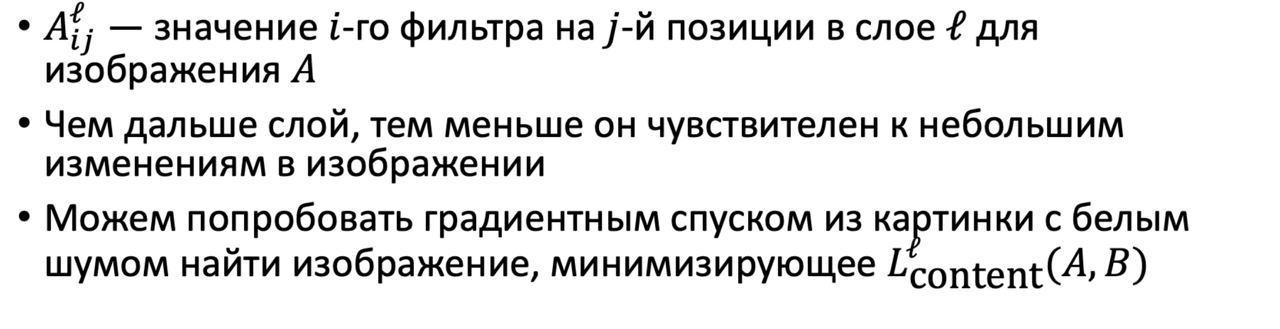
\includegraphics[width=0.7\linewidth]{1_contentnotation.jpg}
\caption{Нотация для первой компоненты Perceptual loss}
\label{fig:1_contentnotation}
\end{figure}
	
	Считаем для слоя l, он конкретный. Прогоняю картинку А в VGG беру слой нейросети l, там i канал (свертка i)  и смотрю ее значение на позиции j (позиция здесь просто индекс для всех возможных положений фильтра на картинке).
	
	Чем больше слой, тем более Loss будет отражать содержательные различия, а не какие-то непонятные мелкие признаки. 
	
	Возьмем значение этого лосса и будем ее минимизировать по B (пиксель), то есть мы будем менять изображение, чтобы добиться наименьшего лосса. 
	
	Лучше брать последние, если нам интересно содержимое. Картинка B меняется попиксельно. 
	
		\subsection{Style}
		
		
			\begin{equation}
	    L^{l}_{style}(A,B) = \sum_{i,j} (G^{l}_{i,j}(A) -G^{l}_{i,j}(B))^{2}
	    \label{eq:1_styletloss}
	\end{equation}
	
	Чтобы посчитать G для A, Мы берем два канала i и j, затем мы рассматриваем k-ю позицию фильтра  на указанных каналах. Перемножаем выходы с филтьтров и суммируем по всем k.
	
	\begin{equation}
	G^{l}_{i,j} (A) = \sum_{k} A^{l}_{i,k} \times  A^{l}_{j,k}
	   \label{eq:1_Gcompon}
	\end{equation}
	
	
	Что по сути происходит в \ref{eq:1_Gcompon}: эта штука показывает то, насколько перекликаются (насколько похожи) i и j канал с точки зрения выходов фильтра, проецируемеого на картинку А. 
	
	Обобщение всего лосса стилевого: он требует, чтобы корреляции каналов между собой (в нашем случае i,j) совпадали для картинки A и картинки B. 
	
	Затем предлагается взять таким образом полученные лосс для отдельных слоев l и просуммировать их с определенными весами. (В этом отличие от контентного лосса, там мы считали для одного слоя, а тут мы складываем по всем слоям). 
	
	
	
			\begin{equation}
	    L_{style}(A,B) = \sum^{L}_{l=0} w_l L^{l}_{style}(A,B)
	    \label{eq:1_styletloss}
	\end{equation}
	
	Как это понимать: 
	
	Допустим, что фильтр 1 детектирует человека (то есть там, тем больше выход, тем больше изображение похоже на человеческое), а фильтр 2 - синий цвет детектирует. Если стилевая картинка в синей гамме, то тогда корреляция между фильтрами будет высокая, поскольку тогда скалярное произведение будет большим. 
	
	Итоговый лосс будет выглядить следующим образом:
	
		\begin{figure}[H]
\centering
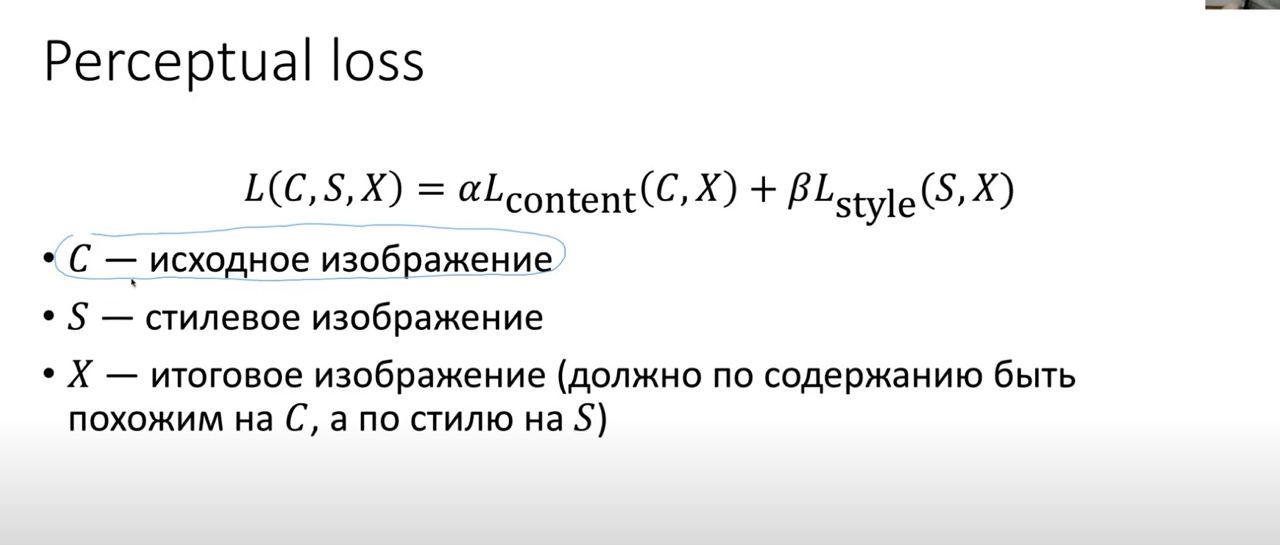
\includegraphics[width=0.7\linewidth]{1_finalloss.jpg}
\caption{Полный лосс}
\label{fig:1_finalloss}
\end{figure}


Нам дается "исходное" изображение, то есть которое мы пытаемся переделать (до этого это был белый шум). Хотим сделать похожим на S. X- результат. Как и с B, мы постоянно обновляем X для уменьшения лосса. $a$ и $\beta$ - гиперпараметры модели.  Минимизируем по X.  
	

	
	\newpage
	\section{Как можно сделать перенос стиля более быстрым, если стилевое изображение известно и не будет меняться?} % S
	В чем вообще проблема: минимизация Perceptual Loss напрямую для каких-то адекватных размеров изображений занимает большое время (порядок времени --- 4 минуты для изображения 1024x1024). Это с точки зрения пользователя плохая история.

В том случае, если стилевое изображение зафиксировано, мы можем не просто напрямую минимизировать Perceptual Loss, а обучить нейросеть на выборке таким образом, чтобы она принимала на вход изображение $x$, а ее выход минимизировал Perceptual Loss.

Изначально было: $L(x, S, \hat{y}) \rightarrow \min\limits_{\hat{y}}$

Теперь стало: $L(x, S, a_\theta(x)) \rightarrow \min\limits_{\theta}$

Здесь $x$ --- входное изображение (пытаемся приблизиться к нему по контенту), $S$ --- стилевое изображение (пытаемся приблизиться к нему по стилю), которое мы и фиксируем, $a_\theta$ --- модель с параметрами $\theta$, принимающая на вход входное изображение и выдающее стилизованное.

То есть фактически мы подбираем модель, которая на выходе бы давала картинку, хорошую с точки зрения Perceptual Loss. Вместо прямой оптимизации мы пытаемся обучить какое-то преобразование.

Подобный подход не позволит нам выиграть времени на обучении (все равно придется обучать сетку, а это требует время), но зато затем, с обученной сеткой, создание картинки с нужным стилем будет значительно быстрее.

Однако, если мы поменяем стилевое изображение, то сетку придется обучать новую (что в целом логично).
	
	\newpage
	\section{3} % Arina
	\section{Что в вариационном автокодировщике выдают кодировщик и декодировщик?} 
	
	Общая идея: 
	
	Обычный автокодировщик кодировал нам как-то картинку в вектора. Этот вектор являлся "характеристиками" этого изображения. 
	
	Хотим чтобы характеристики были не просто какими-то числовыми значениями, но вероятностными распределениями. Этим мы делаем две вещи: включаем в модель неопределенность (пример: плачущий мальчик и Мона Лиза: насчет первого мы точно знаем, что он не улыбается, его распределение будет сдвинуто, а само распределение прижато к среднему, в тоже самое время насчет Мона Лизы мы до конца не понимаем, улыбается она или нет, и раздвигая границы распределения "улыбки" мы этот момент учитываем). 
	
	Задача:
	
	Хотим построить векторное представление картинок $\mathbb{R}^{d}$, но каждая отдельная картинка соответствует не отдельному числу, но распределению определенному в этом векторном пространстве. Следствие: картинка будет описываться не отдельным числом, но некоторой средней и дисперсией нормального распределения. Получившиееся представление есть набор из d распределений со своими средними и дисперсиями. 
	
	Что мы делаем: 
	
	Сэмплируем вектор Z из распределения для картинки x, построеного для конкретной картинки. После этого мой декодировщик берет z и превращает его в $\bar x$.  Добиваемся того, чтобы раскодированная картинка была, как можно ближе к x.
	
	
	\subsection{кодировщик}
	
	Кодировщик представляет картинку в виде набора распределений, которые описываются средним и дисперсией (во время обучения используется логарифм дисперсии). 

	
	\subsection{декодировщик}
	
	Из построенного распределения сэмплируем значения и декодировщик выдает нам картинку, которая похожа на оригинальную. 

	
	\newpage
	\section{4} % Arina
	$\sum\limits^{l}_{i = 1}(\mathbb{E}_{q(z|x_{i})}\text{log} p(x_{i} | z) - \text{KL}(q(z|x) || \mathcal{N}(0,1))) \rightarrow max$ \\ 

$q(z|x)$: q -- это кодировщик (полносвязная или сверточная НС), на вход принимает x (картинку), и выдает z, то есть вектор средних и дисперсий. То есть он выдает распределение представлений при условии, что на вход пришла такая-то картинка. \\ 

$p(z|x)$: p -- это декодировщик. Он принимает на вход скрытый вектор и раскодирует картинку. По сути также представляет собой НС. Декодер выдает нормальное распределение с центром в том, что он раскодировал, плюс $\varepsilon$, то есть некий случайный шум.\\ 

$\mathbb{E}_{q(z|x_{i})}\text{log} p(x_{i} | z)$: взяли распределение на скрытых векторах ('облачко'), из него нагенерили кучу точек. Из каждой этой точки развернули новую картинку ($\tilde x_{1}, \tilde x_{2}, \tilde x_{3}$ и т.д.). Далее оценили, насколько каждая из этих раскодированных картинок похожа на оригинальную. По сути мы тут считаем среднюю ошибку рекострукции. Это слагаемое функционала отвечает за то, что мы хотим, чтобы картинки из распределения были похожи на оригинал (оно называется reconstruction likelihood). \\ 

KL -- это дивергенция Кульбака-Лейблера, мера сходства двух распределений (если KL = 0, то распределения одинаковые). Тут мы просим, чтобы распределение, которым кодируется картинка, было как можно больше похоже на стандартное нормальное. Зачем нам это надо? А затем, что кодировщик очень хочет сделать нам вырожденное распределение, и представить его как точку (то есть сделать распределение с очень узким пиком). Это ведет к переобучению -- тогда декодер заучит, во что нужно развернуть именно эту точку, и картинки не особо будут отличаться между собой. Тогда KL -- это что-то типа регуляризатора в нашем функционале. KL позволяет нам расшакалить распределение, на выходе мы получим что-то с центром в 0, но с дисперсией пошире. Если взять только reconstruction likelihood -- получим пустоты в скрытом вектороном пространстве, все будет описано почти что точками, не понятно будет, во что развернуть какую-то случайно выбранную точку между ними. Если взять только KL -- всякие разные картинки перемешаются между собой, так как они все будут описываться стандартным нормальным распределением. Если вместе -- разные картинки будут друг от друга отстоять, но их распределения будут более размазаны. \\ 

\begin{figure}[H]
	\centering
	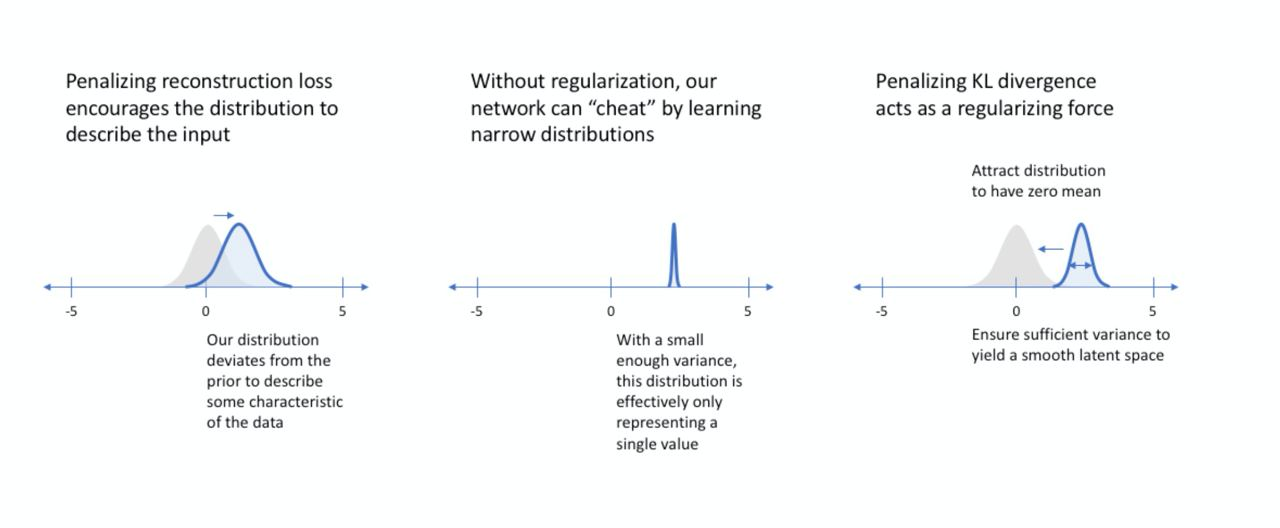
\includegraphics[width=\linewidth]{VAE_loss.jpg}
	\caption{Иллюстрация, что делает KL}
\end{figure}

	
	\newpage
	\section{5} % S
	Кодировщик выдает нам $\mu$ и $\sigma$ и мы по ним генерируем какой-то вектор $z$ из этого распределения. Проблема: непонятно, как посчитать производную производную выхода по $\mu$ и $\sigma$, поскольку там происходит вероятностный процесс. Вместо этого сделаем так:

Кодировщик выдает нам $\mu$ и $\sigma$ (это конкретные детерминированные числа), а еще мы будем генерировать стандартное нормальное число $\varepsilon$. И чтобы получить конкретное представление $z$ мы сделаем $z = \mu + \sigma \odot \varepsilon$ (здесь $\odot$ --- поэлементное умножение). То есть фактически мы разделяем случайность (запихиваем ее в $\varepsilon$), при этом делая ее без параметров (и никакие градиенты туда не нужны), и выдачу параметров кодировщиком (см. рисунок \ref{fig:5_reparameterization} в качестве иллюстрации).

\begin{figure}[H]
	\centering
	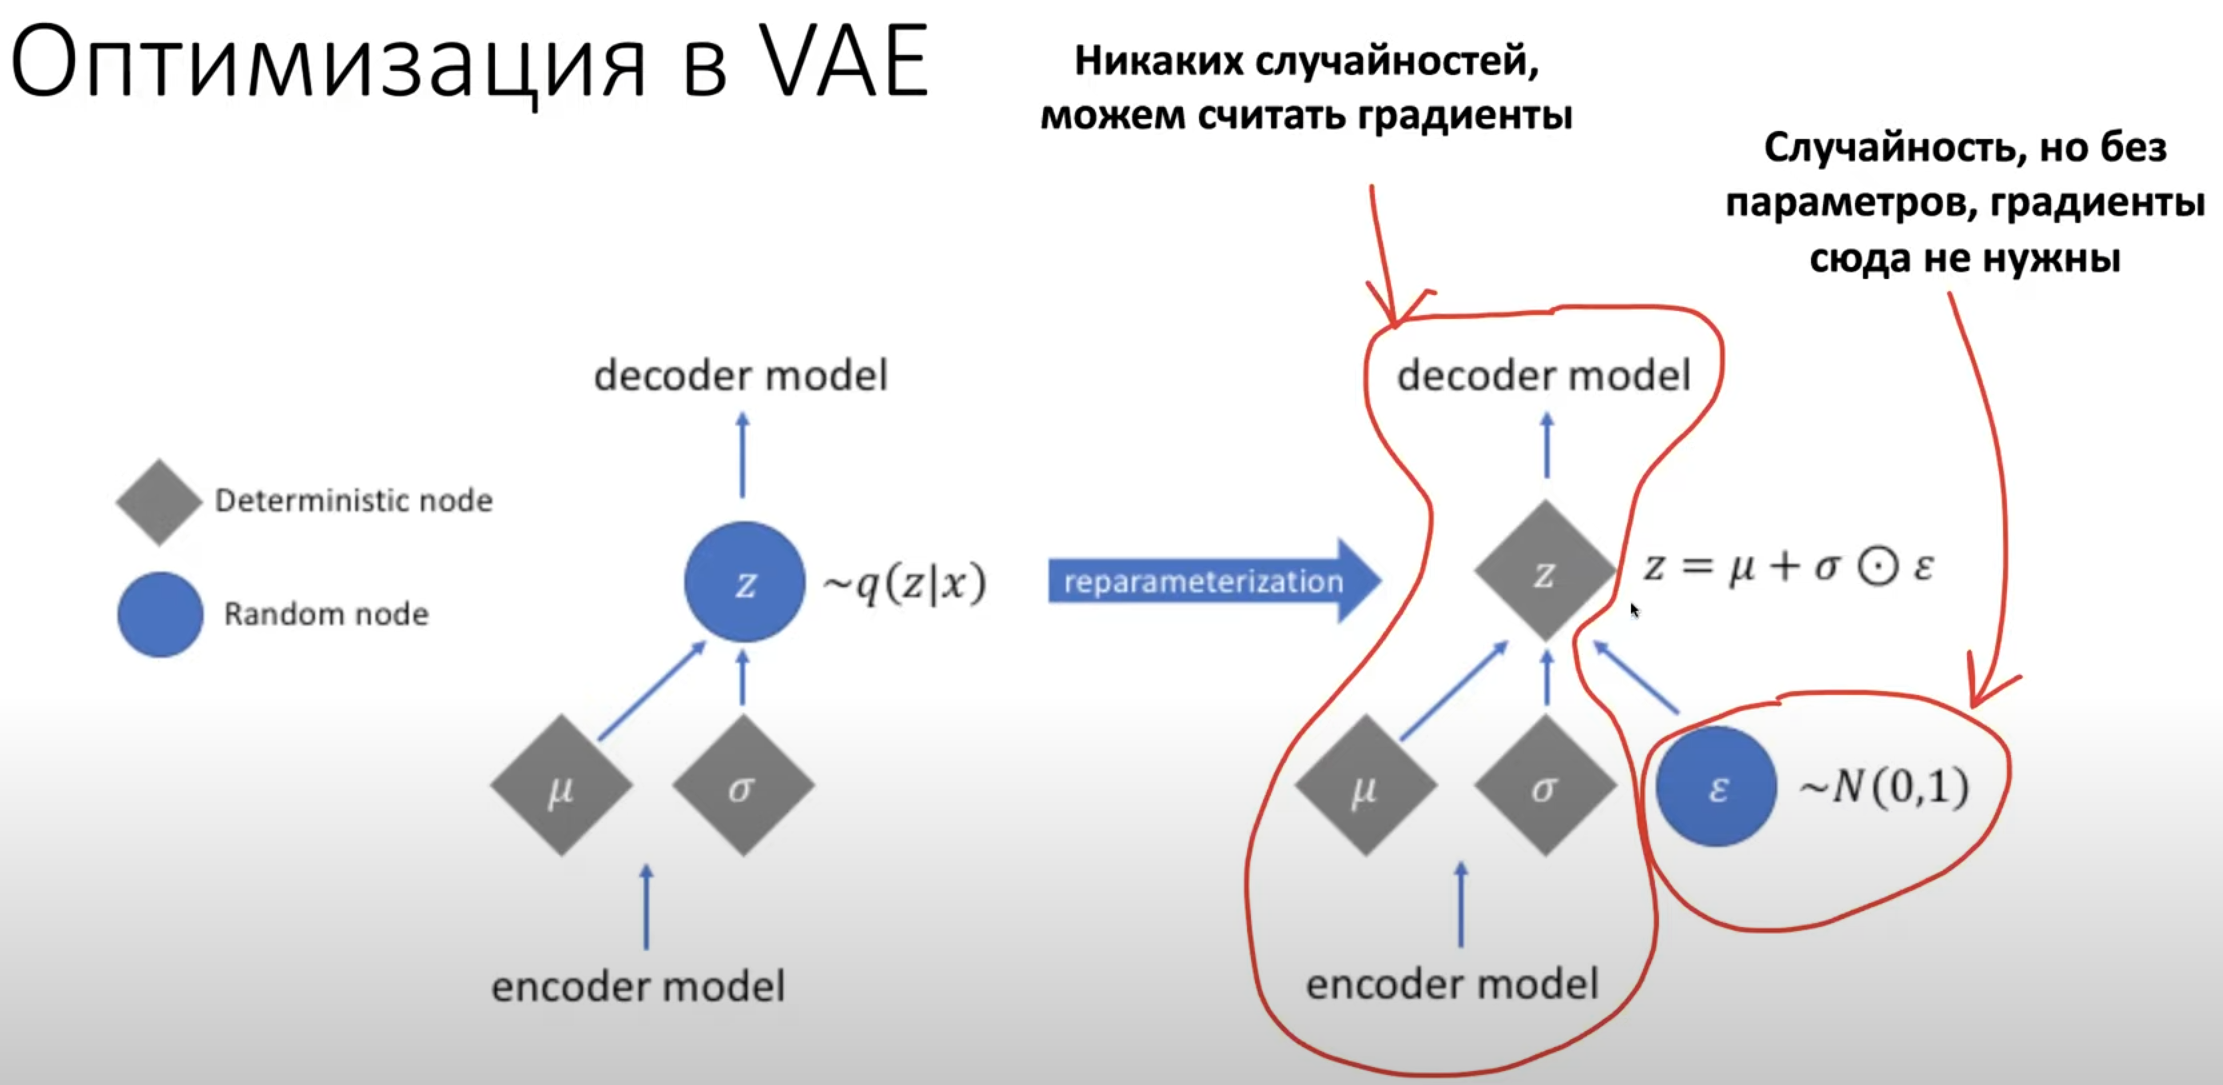
\includegraphics[width=\linewidth]{5_reparameterization}
	\caption{Трюк репараметризации (слева без него, справа с ним)}
	\label{fig:5_reparameterization}
\end{figure}
	
	\newpage
	\section{6} % Arina
	$L(D,G) = -\displaystyle\frac{1}{n}\sum\limits_{x_{i} \in X}log D(x_{i}) -\displaystyle\frac{1}{n}\sum\limits_{z_{i} \in Z}log(1 - D(G(z_{i}))) \rightarrow \max_{G} \min_{D} L(D,G) $ \\

Здесь D -- дискриминатор, G -- генератор. В этой функции потерь мы отдельно считаем ошибку на реальных объектах ($x_{i}$) и сгенерированных объектах ($G(z_{i})$). Сначала мы хотим минимизировать этот функционал на дискриминаторе, хотим научить его лучше разделять объекты. Потом мы максимизируем функционал на параметрах генератора, то есть мы хотим сдвинуть ближе реальные и сгенерированные объекты. \\

При обучении: \\ 
\begin{itemize}\setlength\itemsep{0.2em}
    \item Генерируем n объектов из случайного шума 
    \item Выбираем случайно n реальных объектов \item Берем случайный шум, пропускаем через генератор, передаем это в дискриминатор. Получаем вероятность того, что наши сгенериррованные объекты принадлежат к реальным объектам (и то же самое делаем для самих реальных объектов). 
    \item Используем функцию потерь, чтобы обновить параметры дискриминатора. И так k раз 
    \item Делаем одну итерацию обучения генератора. Еще раз генерим случайный шум и отдаем его дискриминатору, еще раз считаем функцию потерь (при ГС по параметрам генератора нам нужно только второе слагаемое функции потерь, то есть будем смотреть только на то, как хорошо получилось разделить сгенерированные объекты). 
\end{itemize}

Сначала обучаем дискриминатор, он дает нам некую меру сходства (насколько два класса (реальные и сгенерированные изображения) похожи друг на друга). Потом исользуем эту меру сходства, чтобы обучить генератор, чтобы он сдвигался ближе к реальным изображениям. 

	
	\newpage
	\section{7} % S
	Затухание градиентов --- одна из проблем GAN-ов. Предположим, что мы имеем ситуацию, похожую на изображенную на рисунке \ref{fig:7_problem}. В таком случае, как видно, дискриминатор может провести линию так, чтобы идеально (или в целом почти идеально, сути дела не меняет) разделить два класса. Это здорово, но не очень.

Если классы идеально разделились дискриминатором, то $D(x_i) = 1$ для любого $x_i$ в $X$, т.е. для всех объектов первого класса он вернул 1. Для всех же сгенерированных объектов $D(\hat{x_j}) = D(G(z_j)) = 0$ для любого $z_j$~в~$Z$.

Вспомним, как выглядит функция потерь:

\begin{equation}
	L(D, G) = - \frac{1}{n} \sum\limits_{x_i\in X}\log D(x_i) - \frac{1}{n} \sum\limits_{z_j\in Z}\log [1 - D(G(z_j))]
	\label{eq:7_loss}
\end{equation}

Подставим получившиеся значения в функцию потерь \ref{eq:7_loss}:

\begin{equation}
	L(D, G) = - \frac{1}{n} \sum\limits_{x_i\in X}\log 1 - \frac{1}{n} \sum\limits_{z_j\in Z}\log [1 - 0] = 0 = \text{const}
\end{equation}

Константа в том смысле, что нет зависимости от весов генератора или дискриминатора. Это значит, что градиент функции потерь оказывается равным нулю, т.е. ни дискриминатор, ни генератор более не обучаются, поскольку веса не обновляются. Ну понятно, что картинка эта далека от того, чего мы на самом деле хотим, так что это проблема.

\begin{figure}[H]
	\centering
	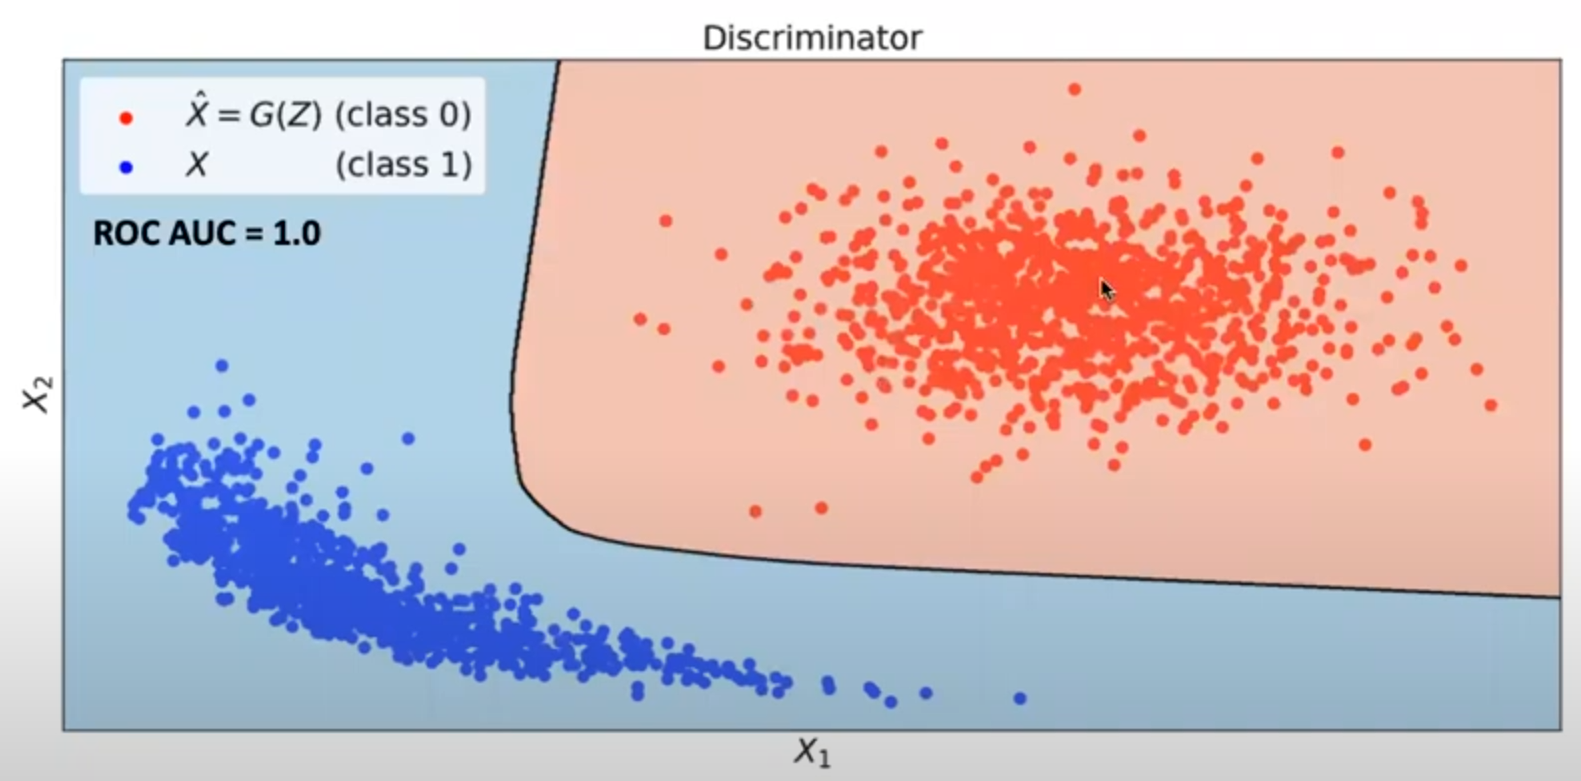
\includegraphics[width=\linewidth]{7_problem}
	\caption{Ситуация, возникшая на некоторой итерации обучения GAN и ведущая к затуханию градиентов}
	\label{fig:7_problem}
\end{figure}
	
	\newpage
	
	\section{8} % S
	\textbf{Теорема (о замене переменных):} \textit{Пусть даны $p_z(z)$ и $z = f(x)$, тогда $p_x(x)$ находится следующим образом:}

\begin{equation}
	p_x(x_i) = p_z(f(x_i)) \left|\det\frac{\partial f(x_i)}{\partial x_i}\right|
	\label{eq:8_theor}
\end{equation}

\textit{где указан определитель матрицы первых производных, которая записывается как:}

\begin{equation}
	\frac{\partial f(x_i)}{\partial x_i} = 
		\begin{pmatrix}
			\dfrac{\partial f(x_i)_1}{\partial x_{i1}}& \dots & \dfrac{\partial f(x_i)_1}{\partial x_{in}} \\
			\vdots & \ddots & \vdots \\
			\dfrac{\partial f(x_i)_m}{\partial x_{i1}}& \dots & \dfrac{\partial f(x_i)_m}{\partial x_{in}} 
		\end{pmatrix}
\end{equation}

Здесь $p_z(z)$ --- распределение $z$, $p_x(x)$ --- функция распределения $x$, $z = f(x)$ --- функция, переводящая $x$ в $z$.

Если говорить на пальцах, то этот модуль определителя в \ref{eq:8_theor} --- отношение объема $\partial z$ к новому объему $\partial x$.

Про матрицу первых производных: т.к. $x$, $z = f(x)$ --- некоторые многомерные векторы, то логично, что у них есть различные компоненты, индексы которых и указываются в матрице первых производных (то есть например левая верхняя компонента это производная первой компоненты $f(x_i)$ по первой компоненте $x_i$).
	
	\newpage
	
	\section{9} % S
	Предпосылка: и $x$, и $z$ имеют размерность $D$.

\subsection{Функция преобразования}

\begin{equation}
	z = f(x) = 
		\begin{cases}
			&z_{1:d} = x_{1:d}\\
			&z_{d+1:D} = x_{d+1:D} \odot \exp[s(x_{1:d})] + t(x_{1:d}) 
		\end{cases}
\end{equation}

Здесь:

\begin{itemize}
	\item $z_{1:d}$ --- первые $d$ компонент вектора $z$;
	
	\item $s(x_{1:d})$ и $t(x_{1:d})$ --- нейронные сети с $d$ входами и $(D-d)$ выходами;
	
	\item $\odot$ --- поэлементное умножение.
\end{itemize}

\subsection{Якобиан}

Матрица первых производных нижнетреугольная и выглядит как-то так:

\begin{equation}
	\frac{\partial f(x)}{\partial x} = 
	\begin{pmatrix}
		\mathbb{I}_d & 0 \\
		\dfrac{\partial z_{1:d}}{\partial x_{1:d}}& \text{diag}\{\exp[s(x_{1:d})]\}
	\end{pmatrix}	
\end{equation}

Но нас интересует на сама матрица, а ее определитель, а он для нижнетреугольной матрицы записывается просто как:

\begin{equation}
	\left|\det \frac{\partial f(x)}{\partial x}\right| = \exp\left[\sum\limits_{j = d+1}^{d} s(x_{1:d})\right]
\end{equation}

\subsection{Обратная функция}

Тут тривиально:

\begin{equation}
	x = f^{-1}(z) = 
	\begin{cases}
		&x_{1:d} = z_{1:d}\\
		&x_{d+1:D} = [z_{d+1:D} - t(z_{1:d})] \odot \exp[-s(z_{1:d})]  
	\end{cases}
\end{equation}
	
	\newpage
	
	\section{10} % Arina
	\begin{figure}[H]
	\centering
	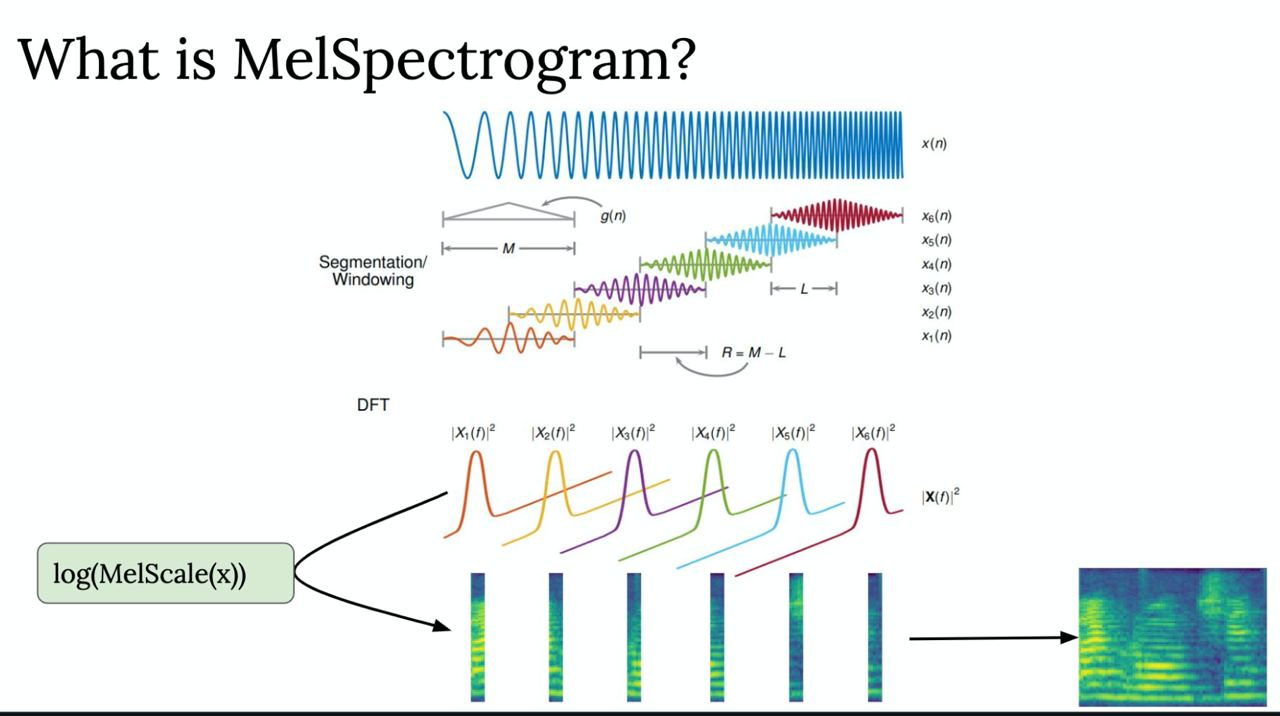
\includegraphics[width=\linewidth]{melspec.jpg}
\end{figure}

Зачем нам вообще спектрограммы? Потому что в одном звуке в сыром сигнале содержится 2000-4000 амплитуд, это дорого хранить. Плюс, мы не инвариантны к шумам и трансформациям. \\

У нас есть исходный сигнал. Мы по нему бежим каким-то окном с каким-то шагом (при этом идем с пересечением -- окна могут накладываться друг на друга). К каждому вырезанному окну мы применяем оконную функцию. Зачем она нужна? На следующем шаге мы будем применять преобразование Фурье, а оно работает с сигналом, который периодичен, то есть он начинается и кончается в нуле (поэтому часто такие фукнции имеют форму 'колокольчика', в домашке например мы применяли косинуисальный фильтр). По сути мы поэлементно перемножаем значение нашего сигнала на значение оконной функции в данной точке. \\ 

Дальше к каждому окошку применяем преобразование Фурье. Суть преобразования Фурье -- представляем сырой сигнал как совокупность синусов и косинусов (например, в форме f(t) = 5 + 2sin(2t + 2) - 3cos(0.2t - 1)). У разных косинусов и синусов будут разные 'веса' и константы. В каждый момент времени каждая отдельная (ко-)синусоида вносит разный вклад в формирование сигнала, веса при них меняются в каждый момент времени. Дискретное преобразование Фурье можно представить как умножение матрицы на окно, которое мы получили на прошлом шаге. Элемент этой матрицы $M_{mn} = exp(-2\Pi i\frac{(m - 1)(n - 1)}{N})$, где N -- длина сигнала. На выходе мы получим вектор той же длины, что исходный, но с мнимыми числами (i.e. от размерности (100,) перешли к размерности (100,2), добавилось второе измерение). \\ 

Далее считаем квадрат комплексной нормы. То есть поэлементно для каждого комплексного числа считаем корень из (квадрат действительной части + квадрат мнимой части). Снова получаем вектор исходного размера (i.e. (100,)). \\ 

Берем первую половину вектора + 1 в силу его симметричности. \\ 

На этом этапе мы получили просто спектрограмму. 
\begin{figure}[H]
	\centering
	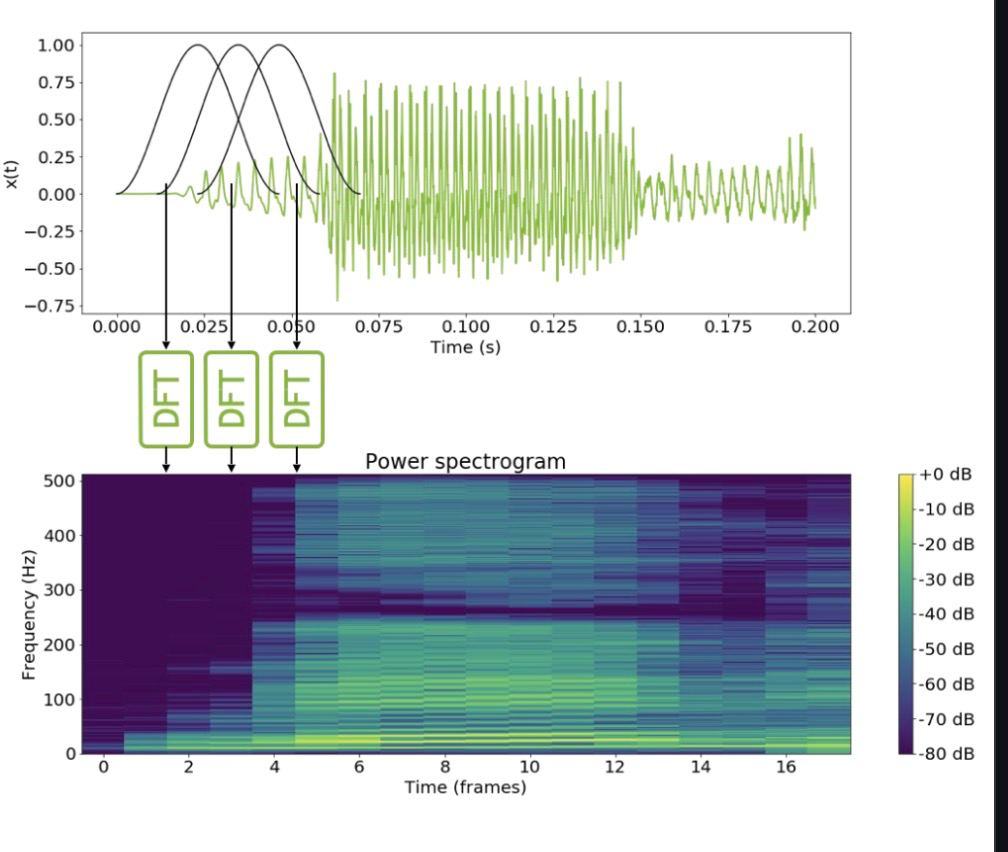
\includegraphics[width=\linewidth]{spec1.jpg}
\end{figure}

Один фрейм (столбик) в спектрограмме -- один раз мы выполнили всю операцию выше. Чем выше идем по столбику, тем более высокие частоты кодируются. Яркость цвета -- насколько в этот момент звучала та или иная частота. Желтый внизу -- это были басы, желтый вверху -- это был писк. \\ 

Как теперь перейти к мелспректрограмме? Для каждого фрейма мы храним все 500 значений частот, хотя часто там наблюдается пустота. Плюс, люди хорошо слышат низкие частоты, а высокие не очень различают. Поэтому мы хотим учесть низкие частоты больше, а высокие -- меньше. Для этого переводим все в мел-шкалу (также реализуемо матричным умножениям). m = 2595 $\log_{10}(1 + \frac{f}{700})$, где f -- значение частоты, а m -- уже значение мелчастоты. Потом еще берем логарифм от мелспектрограммы. \\ 

Эта шкала лучше отражает, что человеческое ухо слышит. Проблема одна -- это преобразование идет не через квадратную матрицу, поэтому восстановить оригинальный сигнал уже не получится. 

	
	\newpage
	
	\section{11}
	\begin{enumerate}
    \item Word Error Rate (WER) -- доля ошибочных слов. 
    
    $WER = \frac{S+D+I}{N}=\frac{S+D+I}{S+D+C}$, где 
    
    \colorbox{Apricot}{S} -- кол-во замен, \colorbox{Aquamarine}{D} -- удалений, \colorbox{Salmon}{I} -- вставок, C -- совпадений.
    
    В примере, где текст "Quick brown fox jumped over a lazy dog" 
    
    был распознан как "Quick \colorbox{Apricot}{brow} \colorbox{Aquamarine}{an} fox jumped over \colorbox{Salmon}{\textcolor{Salmon}{a}} lazy dog" 
    
    $WER = \frac{1+1+1}{8}=\frac{3}{8}$. Процент неправильного распознавания слов речи – это только количественный показатель точности распознавания (количество ошибок распознавания на фразу или слово), но не вероятность распознавания (вероятность неправильного распознавания слова во фразе), потому как он не ограничивается интервалом вероятности $[0; 1]$ и не имеет верхнего предела. Например, представим, что диктор произнес фразу, состоящую из 10 слов, но система ее полностью распознала неправильно и предложила гипотезу из 12 других слов. В этом случае, $WER=120 \%$ $(S=10, I=2, H=D=0)$, и это означает, что показатель точности отрицательный $(-20\%)$, что не имеет смысла с точки зрения теории вероятностей.
    \item CER -- то же самое, но посимвольно. Пробелы считаются. Возможна стратификация или придание весов по типу датасета или тематике.
    \item В Attend \& Spell можно просто посчитать Евклидово расстояние между векторами.
    \item В LAS минимизируем кросс-энтропию.
\end{enumerate}

	
	\newpage
	
	\section{12}
		\section{Что такое MuLaw-кодирование, для чего оно нужно и как оно вычисляется?}
	
	В одном взятом сэмпле обычно находится 16 бит. Это означает, что у нас $2^{16}$ значений. Нам приходится делать softmax на $2^{16}$ значений. Очень много получается, хотим сделать поменьше. 
	
	Рассматриваемый метод позволяет ужать значения амплитуд, сохранив по максимуму первоначальную информацию. 
	
	Интуиция: человеческое ухо слышит в лог шкале: мы хорошо различаем звуки при низких амплитудах и плохо различаем при высоких. Нам надо хранить низкие амплитуды в высоком разрешении, а высокие амплитуды в низком, ибо мы и так их особо не слышим. 
	
	Реализация идеи хороша видна на следующем графике \ref{fig:12_plot}: здесь показано, как звуки с разными амплитудами преобразуются согласно данному кодированию 
	
	
		\begin{figure}[H]
\centering
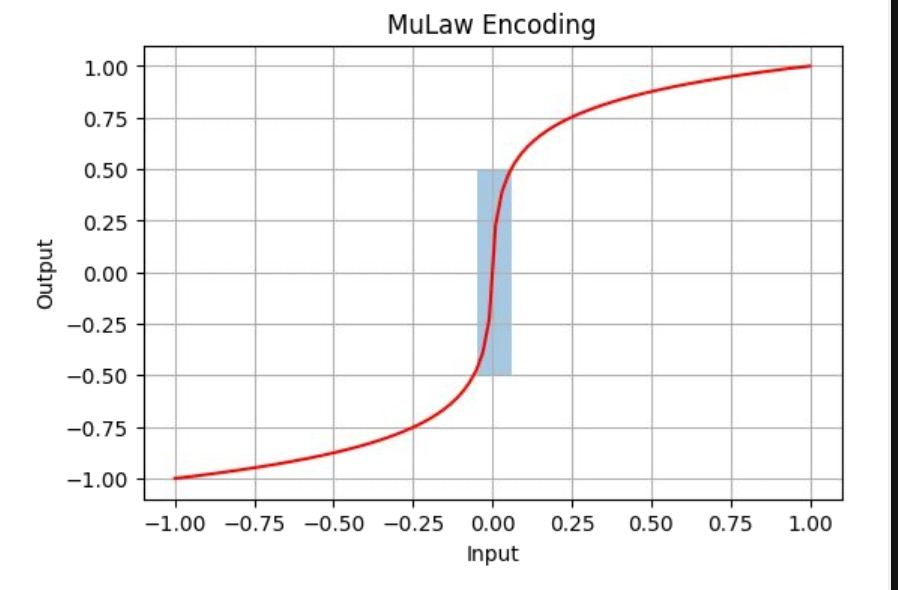
\includegraphics[width=0.7\linewidth]{12_trans.jpg}
\caption{Визуализация Mu law Encoding}
\label{fig:12_plot}
\end{figure}

Как можно увидеть, от -0.1 до 0.1 мы очень компактно храним входные частоты, но чем дальше амплитуда, тем больше у нас становится шаг(скорость функции возрастае), и соответственно в тем меньшем разрешении мы храним звуки с указанной амплитудой. 

Гиперпараметром считается количество конечных значений, в которые мы хотим перевести все наши амплитуды. 


Формула:

\begin{equation}

	    f(x_t) = sign(x_t) \dfrac{ln(1+\mu|x_t|)}{ln(1+\mu)}
	    \label{eq:12_formula}
	    \end{equation}
	
$\mu$ - это просто параметр сжатия ( обычно он вот такой - 255). 

x- нормализованное число, которое подвергается сжатию. 

	
	\newpage
	
	\section{13}
	\begin{figure}[H]
	\centering
	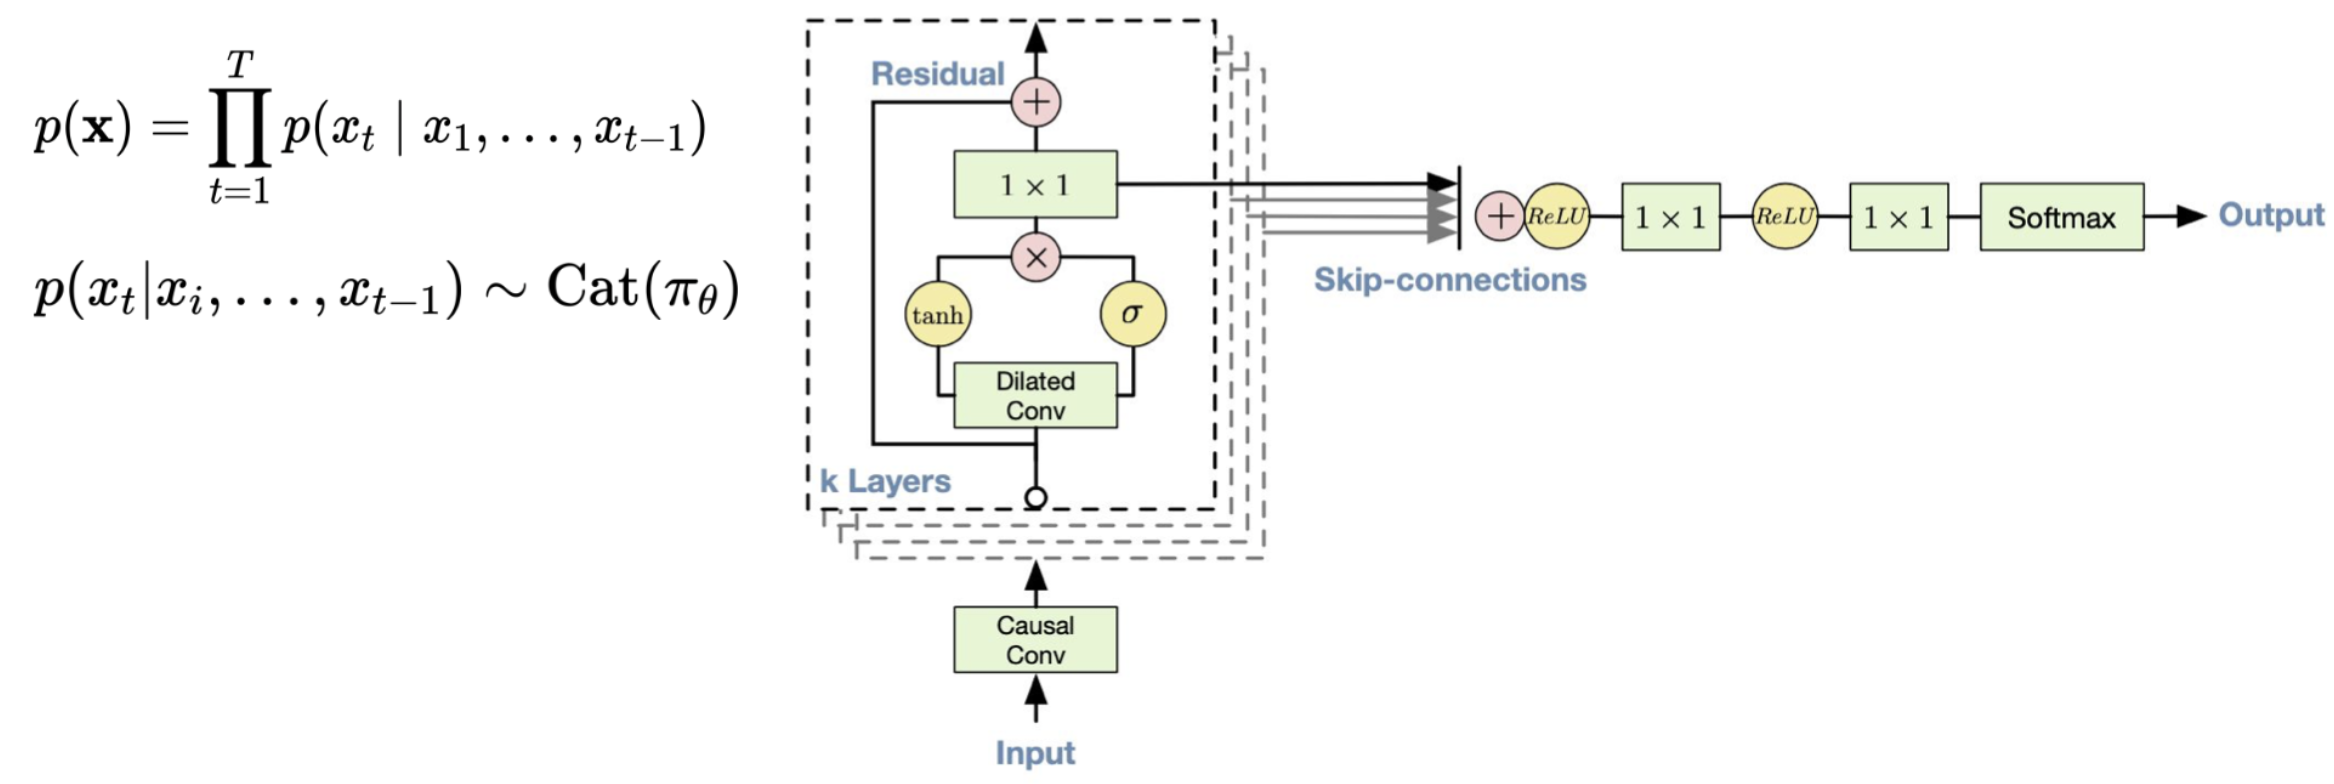
\includegraphics[width=\linewidth]{13_2.png}
	\label{fig:13_2}
\end{figure}


Авторегрессионная модель (моделируем условные вероятности по всем предыдущим сэмплам). Вход -- амплитуды, в train, например, 100 ground truth сэмплов. Для них у нас, например, 12 мелов. Прогоняем через каузальную свертку мелы, растягивая их. Берем первые 99 сэмплов и загоняем в нашу модель. Для каждого сэмпла предсказываем следующий со сдвигом 1. По такой же схеме в строительном блоке (ниже) обуславливаем сэмплы на мелы. Когда будем считать ошибку, возьмем последние 99 сэмплов. Амплитуды проходят через k одинаковых строительных блоков. 


Структура блока:

\begin{figure}[H]
	\centering
	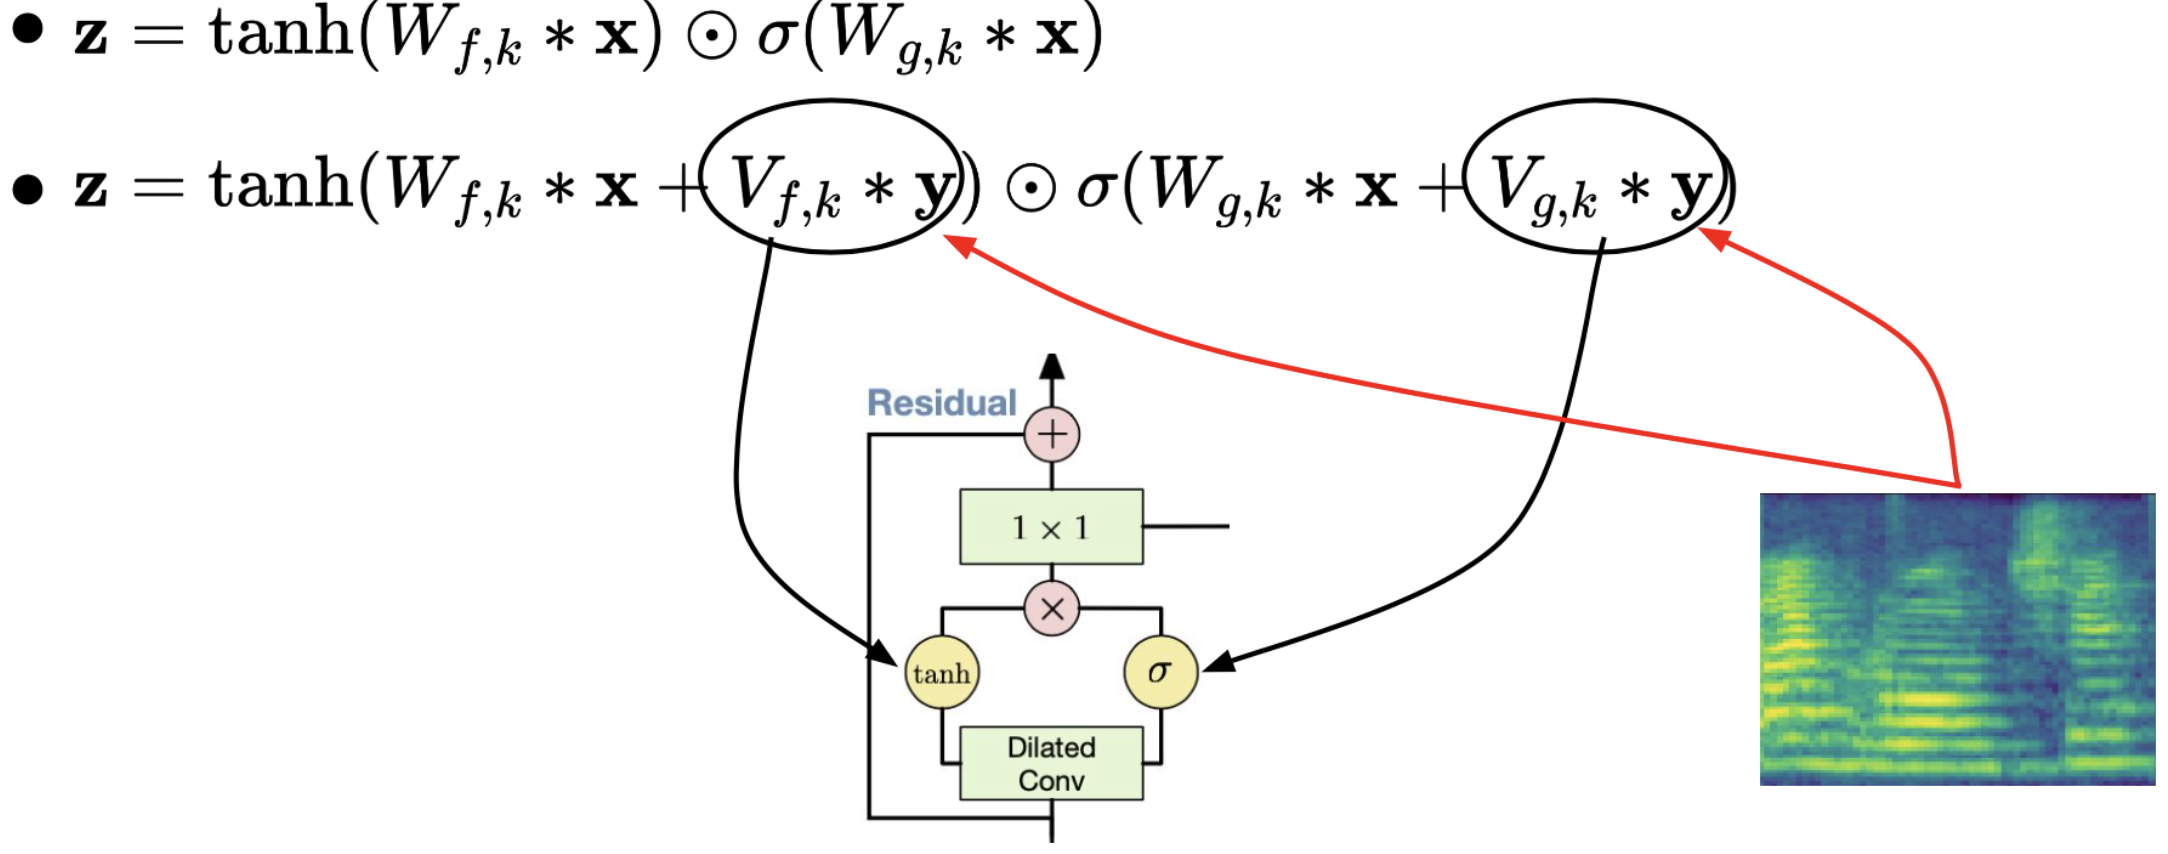
\includegraphics[width=\linewidth]{13_1.png}
	\label{fig:13_1}
\end{figure}



\begin{enumerate}
    \item Каждый сигнал x (на схеме перед dilated conv) сворачиваем двумя каузальными свертками $W_f$ и $W_g$. На каждую кладем сигмоиду и поэлементно перемножаем. Наша сигмоида выучивает, на какие куски аудио смотреть, на какие -- нет. 1 открывает gate внимания, 0 -- закрывает. 1х1 -- свертка с ядром kernel size. Яичко. Это не так важно.
    
    FYI:
    
    Dilated свертки увеличивают рецептивное поле. Dilation растет экспоненциально -- от 1 до 1000 с шагом 2 в каокй-то степени. Рецептивное поле раздувается, что позволяет нам моделировать очень длинные зависимости. Нам это важно, потому что в wav много занимает, но хранит мало информации. Одна секунда -- 16 000 сэмплов. Секунда -- мало, данных -- много.
    
    Второй момент -- каузальные свёртки. Нужны, чтобы моделировать авторегрессию. На стандартной свертке синий -- первый уровень, серый -- второй уровень. На вход синие данные сворачиваем сверткой размером 3 со страйдом 1. Три шарика свернули в один. На самом центральном шарике видно, что он сворачивается, при этом берет вклад и слева, и справа -- смотрит и в прошлую, и в будущее. Нам это не подходит, так как мы не хотим смотреть в будущее. Нам нужно как-то свертку обрубать. Вклад каждого шарика серого или оранжевого цвета или из настоящего, или из будущего. Как делать? Можно добавлять в саму свёртку паддинг. Левый -- правильный, правый -- лишний. Вырезаем его. Можно маскировать свертки. С паддингами проще читать код. 
    
   
    \item Предсказываем, исходя из mel-синтезиса. Сворачиваем mel с двумя свертками (в формуле y -- mel, V -- свертки). Так мы обуславливаем нашу генерацию. Так считаем каждый слой. x и спектрограмма разного размера по времени, и чтобы они совпадали мы должны растянуть спектрограмму до размера сэмпла. Это делается или transpose сверткой, или линейной интерполяцией.
\end{enumerate}

Skip-connections для каждого сэмпла выдает распределение для следующего.

Дальше MuLaw encoding. У каждого представления 16000 сэмплов, и каждый сэмпл -- число. Один сэмпл занимает 16 бит, $2^{16}$ значений. Чтобы софтмакс на таком количестве не ломался, ужимаем амплитуды с сохранением выразительности (см. вопрос 12).

Функция потерь. У нас должно быть какое-то распределение. Чтобы было категориальное, в самом конце на каждый сэмпл навешиваем softmax и предсказываем вероятность той или иной амплитуды. Но в целом нам ничего не мешает использовать нормальное распределение. Или смесь распределений.

Почему медленно: каузальные свертки. Мы делаем что-то для каждого сэмпла отдельно, т. к. следующий зависит от предыдущего. Усовершенствованные сетки работают с несколькими сэмплами одновременно. Например, изначально кормятся белым шумом:


\begin{figure}[H]
	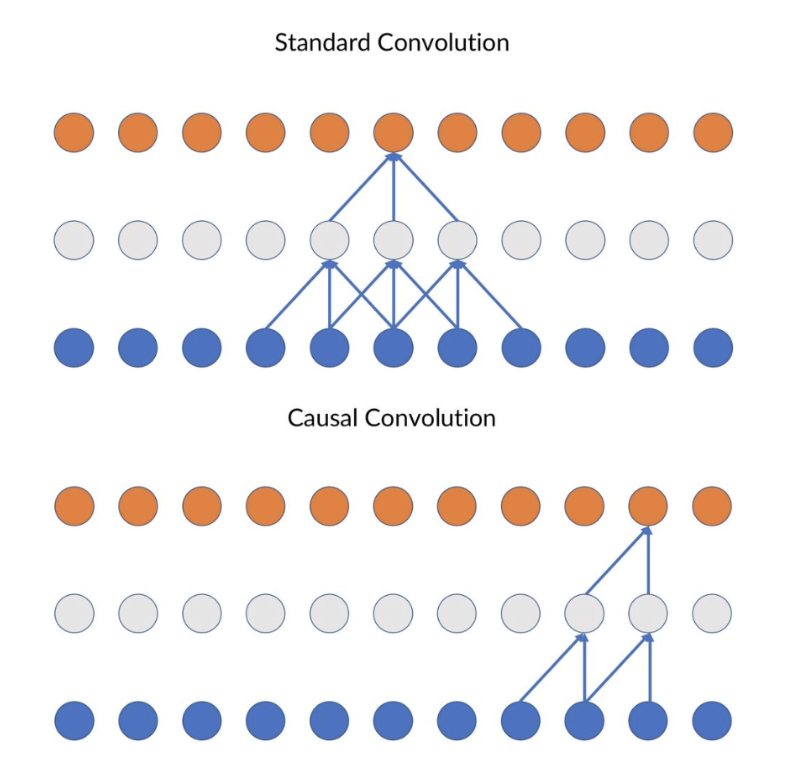
\includegraphics[width=0.5\linewidth]{13_4.png}
	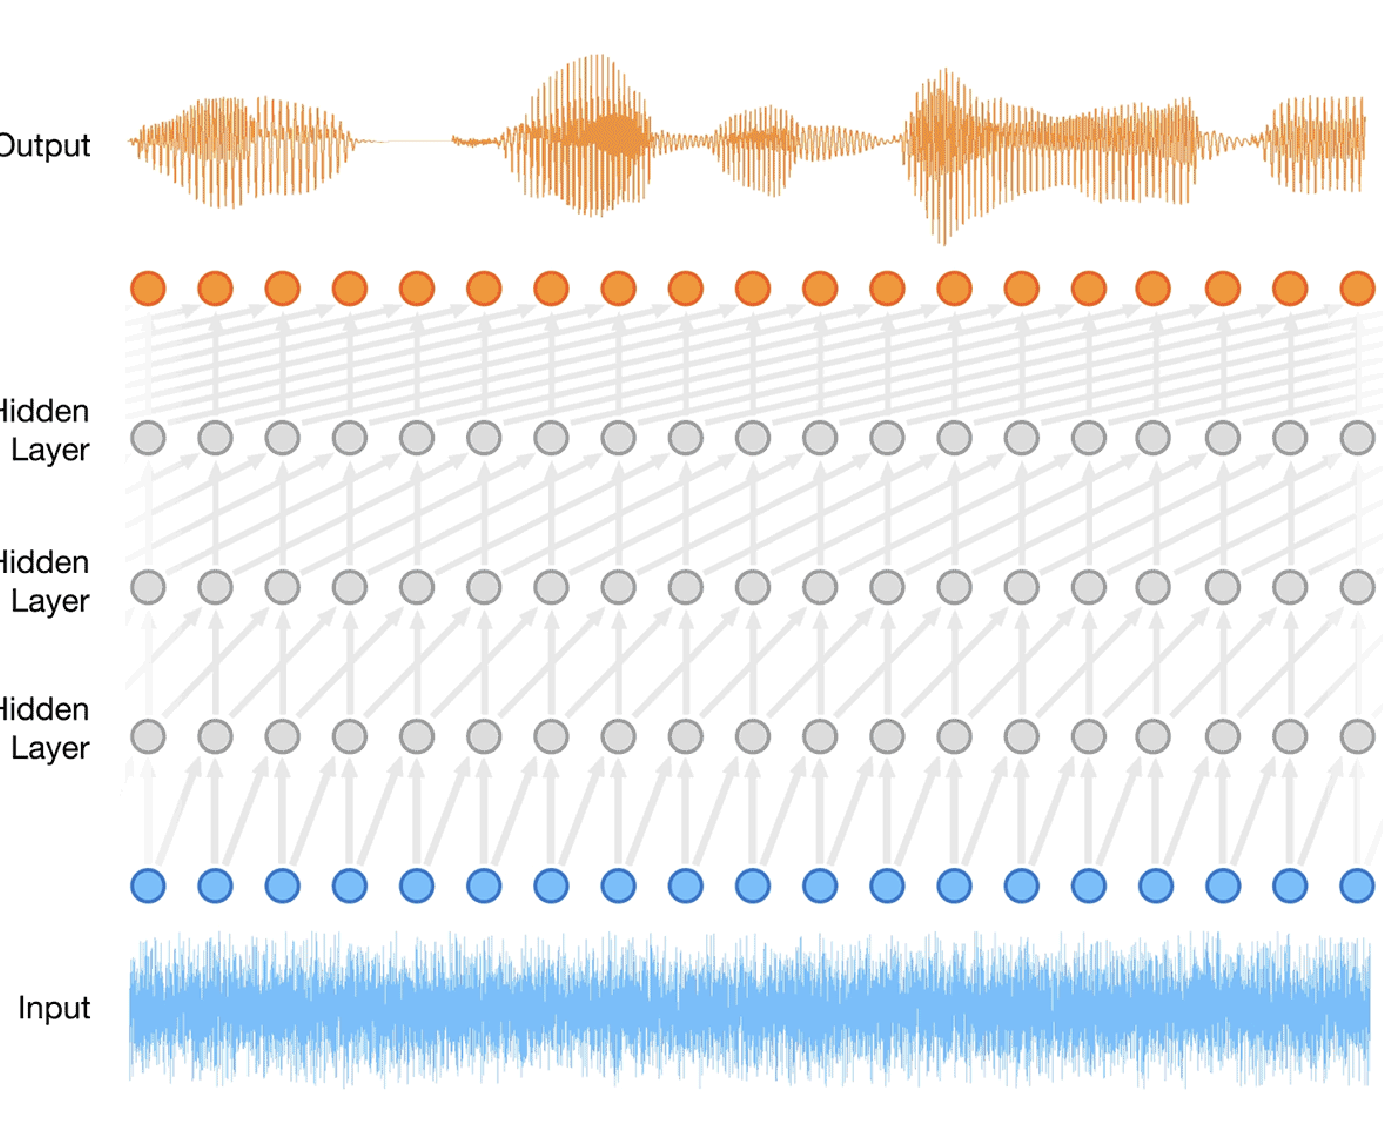
\includegraphics[width=0.5\textwidth]{13_3.png}
	\label{fig:13_3}
\end{figure}

	
	\newpage
	
	\section{14}
	Поступает пара $(u, i)$ -- user, item. 

По ней считаем какие-то признаки $x^{u, i}_1, ... x^{u, i}_\alpha$. Например, сколько лайков u поставил всем видео этого автора; как много видео с такими же тегами просмотрены; отношение всех кликов ко всем просмотрам это видео. 

Обучающая выборка -- R, набор признаков для всех известных пар $(u, i)$.

Рейтинг -- какая-то оценка результата взаимодействия пользователя u с айтемом i. Это может быть вещественное число, например, рейтинг, поставленный фильму, от 1 до 10. Может быть что-то бинарное -- поставил или не поставил лайк. Что-то категориальное -- в фейсбуке может быть лайк с разными реакциями. Множество необязательно будет упорядоченным.

	
	\section{15} % Arina
	Если рейтинги вещественные, то можно свести к задаче регресии. Тогда метрики будут MSE, MAE, RMSE и так далее. Если же мы сводим к задаче классификации, также можно взять знакомые метрики вроде F-меры, AUC ROC и т.д. Но рекомендательная система же выдает какое-то ограниченное число айтемов (и нам важно, что находится именно в топе наших рекомендаций). Тогда предполагаем, что рек.система выдает ранжированный список айтемов, и будем считать, что мы показываем пользователю top-k рекомендаций. Поэтому на этом числе k мы и будем считать качество. \\ 

hitrate@k = [$R_{u}(k) \cap L_{u} \ne \varnothing$], где $R_{u}(k)$ – наши top-k рекомендаций, $L_{u}$ -- айтемы, которые пользователю действительно понравились. То есть это индикатор того, что хотя бы 1 из наших рекомендованных айтемов понравился пользователю. \\ 

precision@k = $\frac{|R_{u}(k) \cap L_{u}|}{k}$ -- сколько айтемов из тех, что мы порекомендовали, пользователю действительно понравилось. \\ 

recall@k = $\frac{|R_{u}(k) \cap L_{u}|}{|L_{u}|}$ -- показыыает, насколько мы смогли вытянуть в топ релевантный контент. \\ 

Есть метрики более специфичные для рекомендаций -- это метрики качества ранжирования. Неплохо было бы учитывать, в каком порядке мы выдаем рекоемндации (айтемы, которые по идее должны сильно зайти пользователю, должны идти первыми, например). \\ 

Пусть $a_{ui} = a(u, i)$, то есть предсказание нашей системы по этому юзеру и по этому айтема. Далее мы сортируем айтемы по возрастанию $a_{ui}$ для конкретного юезра u (и берем первые k рекомендаций). Тогда для этого списка рекомендаций посчитать меру DCG, которая будет накидывать штраф за позицию айтема в ранджировании. \\ 

DCG@k = $\sum\limit_{p = 1}^{k} g(r_{uip})d(p)$ \\ 

p -- номер позиции в ранжировании, $r_{uip}$ -- оценка, которую пользователь u поставил айтему на позиции p (истинные рейтинги). $g(r_{uip}) = 2^{r} - 1$ или $g(r) = r_{uip}$.  $d(p) = \frac{1}{log(p + 1)}$, это как раз штраф за позицию. Например, если у нас взаимодействие может принимать только значения 0 и 1 (например, был клик или нет), то мы просто будем складывать 1/log(1 + p), и эта сумма будет больше, если единички у нас оказываются в начале списка рекомендаций. \\ 

Можно посчитать еще normalized DCG@k(u) = $\frac{DCG@k(u)}{maxDCG@k(u)}$. \\

Как еще можно измерить качество рекомендательных систем? \\ 
1. Novelty (число айтемов, которые раньше пользователю не рекомендовали) \\ 
2. Разнообразие. Можно посчитать расстояние между эмбеддингами айтемов, которые мы порекомендовали. Или использовать метаинформацию об айтемах (жанры, исполнители) и посчитать ее дисперсию. \\ 
3. Serendipity -- умение рекомендовать редкие айтемы, которые пользователю заходят. Например, b -- новая книга, B -- множество книг, которые пользователь уже оценил, $C_{Bw}$ -- число книг автора w в множестве B, $C_{B}$ -- максимальное число книг одного автора в B. Тогда мы можем измерить сходство между b и B. \\ 
d(b, B) = $\frac{1 + C_{B} - C_{Bw}}{1 + C_{B}}$ \\ 
То есть рекомендация будет новее, если юзер еще не видел айтемы этого автора/испольнителя/etc.

	
	\newpage
	
	\section{16} 
	Ссылка на оригинальный конспект: \url{https://github.com/hse-ds/iad-applied-ds/blob/master/2020/lectures/lecture01-recommender.pdf}
	
	Как понять, что пользователю может понравиться товар? Первый вариант — поискать похожих на него пользователей и посмотреть, что нравится им; также можно поискать товары, похожие на те, которые этот пользователь уже покупал. Методы коллаборативной фильтрации строят рекомендации для пользователя на основе похожестей между пользователями и товарами, которые похожие пользователи выбирают.
	
	Сначала необходимо определить, что пользователи похожи между собой. Для этого считается корреляция Пирсона. 
	
	Далее мы можем посчитать сходство товаров исходя из тех рейтингов, что рассматриваемые два пользователя им поставили. 
	
	Эти формулы определения похожести между пользователями приведены здесь:
	
\begin{figure}[H]
\centering
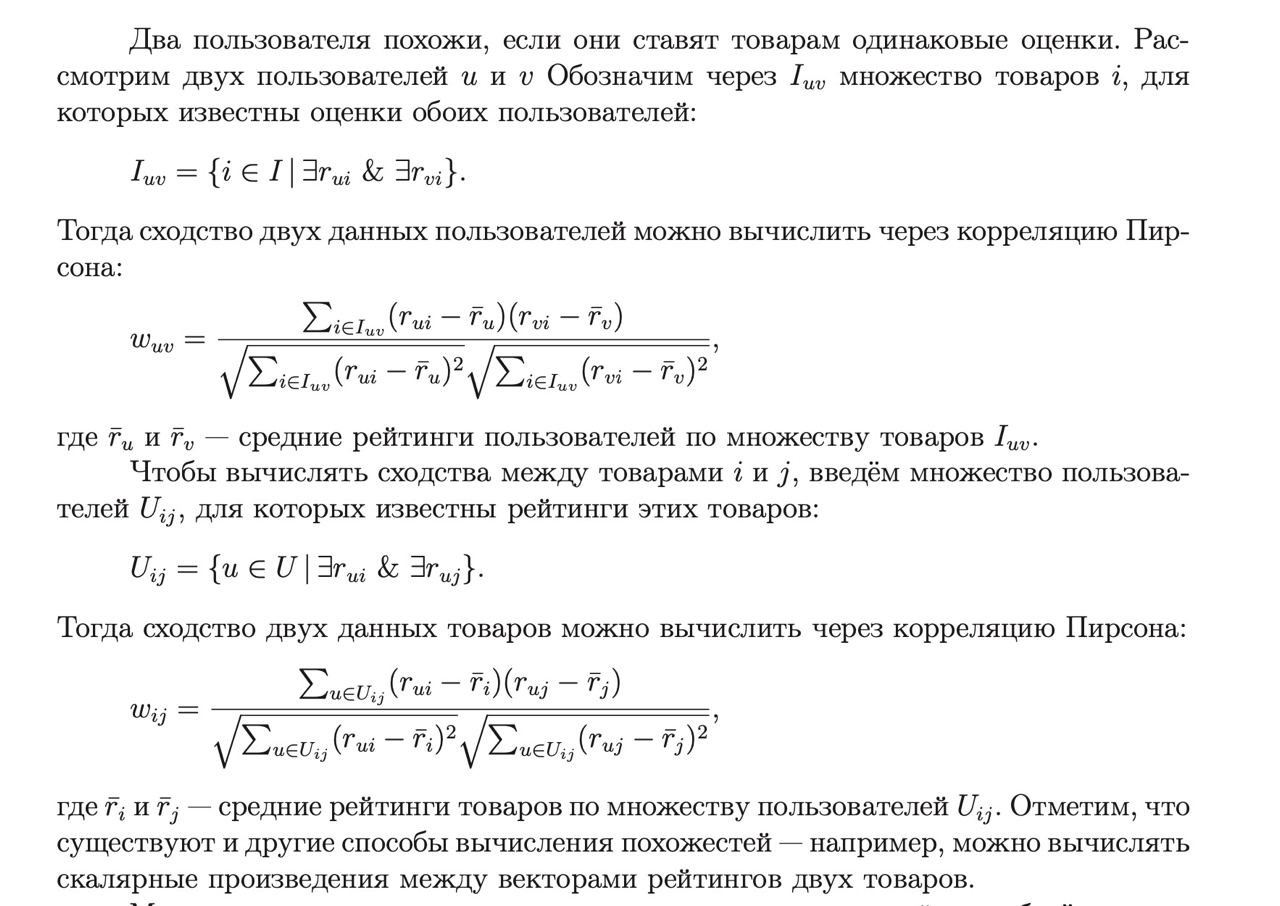
\includegraphics[width=0.7\linewidth]{16_memory1.jpg}
\label{fig:16_memory1} 
\caption{Формулы для определения похожести пользователей}
\end{figure}
	
	
	После того, как мы определили степень похожести товаров между собой и пользователей между собой, нам нужно понять, какие все-таки товары нам рекомендовать пользователю.
	
	Здесь существует два подхода:
	
	1) user-based collaborative filtering 
	
	2) item-based collaborative filtering 
	
	В основе первого подхода лежит процедура, согласно которой мы определяем множество похожих пользователей $U(u_0)$: $U(u_0) = \{v \in U | w_{u_0 v} > \alpha\}$. Эта штука называется коллаборацией, то есть множество похожих пользователей, которые (примерно) одинако оценивают продукты. 
	
	Дальше рекомендуем пользователи те продукты, которые он сам не оценил, но которые хорошо оценили пользователи из коллаборации. 
	
	Для этого мы считаем, как часто товар покупался пользователем из множества $U(u_0) $
		

	
			\begin{figure}[H]
\centering
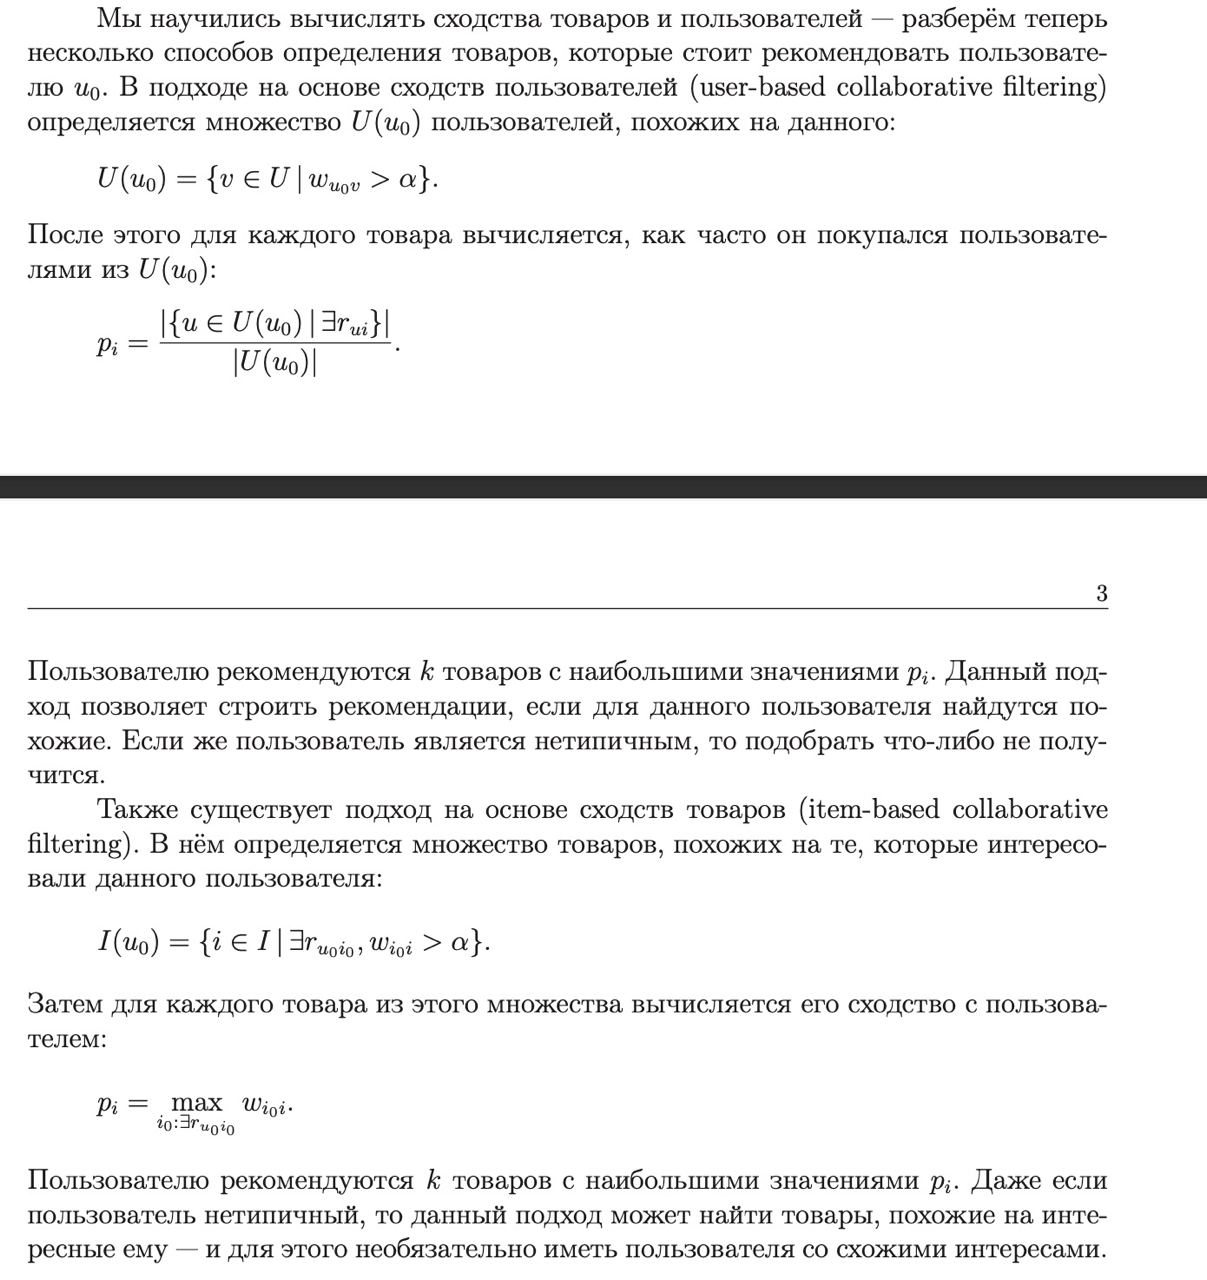
\includegraphics[width=0.7\linewidth]{16_memory2.jpg}
\caption{Формула рассчета частоты покупки товаром пользователями из коллаборации}
\label{fig:16_memory2} 
\end{figure}

	
	\newpage
	
	\section{17} % Arina
	Для каждого пользователя мы имеем d-мерный вектор $p_{u}$, для каждого айтема -- d-мерный вектор $q_{i}$. Мы хотим, чтобы $<p_{u}, q_{i}> \approx r_{ui}$, то есть чтобы скалярное произведение этих векторов аппроксимировало истинный рейтинг. \\ 

В вольной интерпретации (с лекции) можно представить, что d -- это число жанров вообще среди наших айтемов. В $p_{u}$ мы имеем набор оценок, насколько юзеру нравится каждый из жанров, а в $q_{i}$ -- распределение жанров в конкретном айтеме. Тогда $<p_{u}, q_{i}>$ -- мера сонаправленности, чем больше метч между юзером и айтемом, тем больше скалярное произведение. По факту конечно внутри векторов не жанры и предпочтения юзеров, а какие латентные неинтерпретируемые факторы, которые рек.система сама выделила. \\ 

Функционал: $\sum\limits_{(u, i, r_{ui}) \in \mathbb{R}}(r_{ui} - b_{u} - b_{i} - <p_{u}, q_{i}>)^{2} \rightarrow min_{b_{u}, b_{i}, q_{i}, p_{u}}$  \\ 

То есть мы не просто считаем квадратичную ошибку между истинным рейтингом и нашей аппроксимацией скалярным произведением векторов, но и отнимаем из истинного рейтинга среднюю оценку пользователя на всех айтемах ($b_{u}$) и среднюю оценку этого айтема ($b_{i}$) (т.к., например, какие-то юзеры всем ставлят только 4-5 звездочек, и для них 4 это скорее плохо, а кто-то очень сильно придирается, и для них 4 это круто). По сути в этом функционале мы обучаем оба элемента скалярного произведения -- и вектор пользователя, и вектор айтема. Еще к этому функционалу можно накинуть регуляризацию (потребовать, чтобы нормы векторов были не очень большими) ($\lambda\sum||p_{u}||^{2} + \mu\sum||q_{i}||^{2}$).  \\ 

В чем тут есть проблема? Мы тут перемножаем параметры, которые обучаем, это плохо (функция не выпуклая, локальные минимумы появляются и все такое). \\ 

По факту у нас есть матрица P, где лежат все вектора для пользователей, и матрица Q, где лежат все вектора для айтемов, и мы пытаемся осуществить приближение $P^{T}Q \approx R$. \\ 

Как обучаем? \\ 
1) SGD. На каждой итерации берем случайные пары u, i, $r_{ui}$. Но это довольно плохо работает \\ 
2) Alternating Least Squares (ALS). Как-то инициализируем матрицы P и Q. Далее фиксируем Q, обучаем на функционал. Тогда вектора $q_{i}$ оказываются фиксированы, они типа как постоянные признаки, а вектора $p_{u}$ -- это типа как веса при признаках. Получается что-то вроде линейной модели. И так для каждого пользователя мы натрасиваем вектор p. Потом фиксируем матрицу P и подбираем вектора в Q и вот так шаги меняются. \\ 
Это работает лучше, так как при фиксированнии части скаларного изображения получается нормальная линейная выпуклая функция (как в обычных линейных моделях). \\ 

Практический нюанс (хз надо или нет но пусть будет). Потоянно обновлять матрицы вычислительно тяжко. А айтемов у нас обычно сильно меньше, чем пользователей. Тогда мы можем хранить только сравнительно небольшую матрицу Q. При появлении нового юзера подбираем для него $p_{u}$ при фиксированном Q, и делаем рекомендацию через $<p_{u}, q_{i}>$ (делаем один шаг в ALS).  То есть векторы айтемов мы фиксируем, а векторы пользователей постоянно дообучаем на основе последних действий. Раз в сутки/неделю/месяц/хз полностью осуществляем ALS и обновляем матрицу Q тоже. 

	
	\newpage
	
	\section{18} 
	Нужна для учета неявной информации.

Бывают ситуации, когда рейтинги специфичные. Например, для пар $u, i$ мы либо знаем, что взаимодействие было, либо не знаем ничего. Например, мне отгрузили информацию про то, как пользователи ходят по интернету. Я знаю, что он там только был. Не знаю, понравилось ли ему. Или человек как овощ смотрел Netflix -- и что с ним делать? Целевая переменная принимает одно значение, и другие модели can't help. Есть iALS -- implicit alternating least squares. 

Ввожу показатель $S_{u,i} = 1$ (взаимодействие было) или 0 (не было). И показатель $C_{u, i}=\alpha$ , если $S_{u,i}=1$, и 1 в обратном случае. $\alpha \sim$ 50

Изначально все i, с которыми пользователь взаимодействовал -- положительный пример. Нет -- отрицательный. Но это неправильно. Вдруг они понравятся пользователю, когда увидит? Поэтому мы просто учитываем отрицательную информацию с очень маленьким весом. За это отвечает $C_{u, i}$. Так я создаю себе второй класс i, с которыми пользователь не взаимодействовал. 

Суммируем $C_{u, i}$ по всем айтемам, аналогично LFM:

\begin{equation}
    \sum^{n}_{u=1}\sum^{m}_{i=1}C_{u, i}(S_{u, i} - b_i - b_u - < p_u, q_i > )^2 \rightarrow \min b_u, b_i, p_u, q_i 
    \label{eq:18_theor}
\end{equation}

	
	\newpage
	
	\section{19} 
	В рекомендательной системе может участвовать очень большое количество то- варов. При каждом посещении пользователем веб-страницы, где есть блок рекомендаций, необходимо выдать ему k наиболее подходящих товаров, причём достаточно быстро (пользователь не может ждать минуту, пока загрузится страница). В хоро- шей рекомендательной системе участвуют сотни признаков — их вычисление для каждого товара, а затем ещё и применение ко всем товарам градиентного бустинга или графа вычислений вряд ли получится успеть сделать за 1 секунду. Из-за этого рекомендательные системы работают в несколько этапов: обычно всё начинается с отбора кандидатов, где быстрая модель выбирает небольшое количество (тысячи или десятки тысяч) товаров, а затем только для этих товаров вычисляется полный на- бор признаков и применяется полноценная модель. В качестве быстрой модели может выступать линейная модель на нескольких самых важных признаках или, например, простая коллаборативная модель.

\subsection{Отбор кандидатов}

Отбор кандидатов это про то, как выбрать подмножество предметов, которые пользователю интересны. 

\begin{itemize}
	\item те же предметы, производители, что и в истории пользователя 
	
	\item самое популярное сейчас
	
	\item Матричное разложение: пользователь - исполнитель. $r_{user, singer} \approx <p_{user}, p_{singer} >$
	
	\item на основе сходства: $p_{user}, q_{item}$  -  эмбеддинги (например, из LFM). Ищем K items с максимальным значением скалярного произведения $<p_{user}, q_{item}>$. Ищу вещи, которые ближе всего к пользователю. 
	
	
\end{itemize}


О ранжировании  смотрите здесь
\url{https://developers.google.com/machine-learning/recommendation/dnn/re-ranking}

и здесь \url{https://github.com/hse-ds/iad-applied-ds/blob/master/2020/lectures/lecture03-recommender.pdf}

После отбора кандидатов следует ранжирование

Переранжирование - помимо максимизации вероятности клика, мы хотим учесть бизнес-требования. Например, мы не хотим показать видео от одного и того же автора. Мы пересортировываем наш изначальное ранжирование. Так мы учитываем дополнительные требования к нашей рекомендациии. 

\end{document}
